\chapter{Použité metody}

% korelace
% ortogonální

\section{Analýza hlavních komponent}

Analýza hlavních komponent (anglicky \emph{Principal Component Analysis}, dále jako PCA) je metoda používaná pro extrakci proměnných, redukci vícedimenzionálních dat nebo vizualizaci dat.

Jednotlivá pozorování obsažená v datech bývají popsána několika různými proměnnými. Tyto proměnné jsou často vzájemně korelované a obsahují šum. Metoda PCA umožňuje extrahovat pouze důležité informace z proměnných a snížit šum. K tomu je třeba vypočítat nové ortogonální proměnné, nazývané hlavní komponenty, které se získají jako lineární kombinace původních proměnných \cite{bib:PCA1}. Hlavní komponenty reprezentují směry největšího rozptylu původních dat, jinými slovy se jedná o přímku,  které nesou největší informaci o datech. Hlavní komponentu si lze představit jako novou osu, která umožňuje vidět data v takovém rozložení, že rozdíly mezi pozorováními jsou lépe patrné.  %https://builtin.com/data-science/step-step-explanation-principal-component-analysis

\subsection{Princip}

Předpokládáme množinu dat $X = (\bm{x}_1, \ldots, \bm{x}_N )$, kde $N$ j počet pozorování a každý vektor $\bm{x}_i$ přísluší jednomu pozorování popsanému $M$ proměnnými. $\mathbf{X}$ je potom matice rozměru $N\times M$ vstupních dat. Dále je definovaný výběrový průměr $\bar{\bm{x}}$ jako
\begin{equation}
    \bar{\bm{x}} = \frac{1}{N} \sum_{i=1}^{N} \bm{x}_i,
\end{equation}
a výběrová kovarianční matice $\mathbf{C}$

\begin{equation}
    \mathbf{\mathbf{C}} = \frac{1}{N} \sum_{i=1}^{N} (\bm{x}_i - \bar{\bm{x}}).
\end{equation}

První hlavní komponentu, která popisuje největší rozptyl dat označíme $y_{1i}$ a vypočteme následovně jako lineární kombinaci původních proměnných
\begin{equation}
    y_{1i} = \bm{a}_1^\top (\bm{x}_i - \bar{\bm{x}}), \quad \mbox{pro } i=1,\ldots,N,
\end{equation}
kde $\bm{a}_1 = (a_{11}, \ldots, a_{M1})^\top $ je vektor vah. 

Optimální vektor $\bm{a}_1$ je takový vektor, který maximalizuje výběrový rozptyl nové proměnné $y_{1i}$ za podmínky $\bm{a}_1^\top\bm{a}_1 = 1$. Pakliže je výběrový rozptyl $y_{1i}$ definován jako 
\begin{equation}
    D(y_{11}, \ldots, y_{1N}) = \bm{a}_1^\top \mathbf{C} \bm{a}_1
\end{equation}
můžeme maximalizační úlohu vyřešit pomocí metody Lagrangeových multiplikátorů. Lagrageova funkce s parametrem $\lambda_1$ má následující tvar
\begin{equation}
    \mathcal{L}(\bm{a}_1, \lambda_1) = \bm{a}_1^\top \mathbf{C} \bm{a}_1 - \lambda_1(\bm{a}_1^\top\bm{a}_1 - 1).
\end{equation}

Derivaci funkce položíme rovnou nule 
\begin{align*}
    \frac{\partial \mathcal{L}}{\partial \bm{a}_1}  = 2 \mathbf{C} \bm{a} - 2\lambda_1 \bm{a}_1 \overset{!}{=}  0 \\
    (\mathbf{C} - \lambda_1 \mathbf{I} ) \bm{a}_1 \overset{!}{=}  0,  \\
\end{align*}
kde $\mathbf{I}$ je jednotková matice.

Řešíme soustavu lineárních rovnic pro neznámý parametr $\bm{a}_1$, která má řešení právě tehdy, když je matice $\mathbf{C} - \lambda_1 \mathbf{I} $ singulární, tedy platí, že její determinant  je roven nule. $\lambda_1$ je pak největší vlastní číslo matice $\mathbf{C}$ a $\bm{a}_1$ vlastní vektor příslušný tomuto vlastnímu číslu. Toto tvrzení se matematicky zapíše následovně
\begin{equation}
    \mathbf{C} \bm{a}_1 = \lambda_1 \bm{a}_1. \\
\end{equation}
Po vynásobení vektorem $\bm{a}_1$ zleva získáme řešení pro maximální rozptyl proměnné $y_{1i}$
\begin{equation}
    D(y_{11}, \ldots, y_{1N}) = \bm{a}_1^\top \mathbf{C} \bm{a}_1 = \lambda_1.
\end{equation}


Druhá hlavní komponenta
\begin{equation}
    y_{2i} = \bm{a}_2^\top (\bm{x}_i - \bar{\bm{x}}), \quad \mbox{pro } i=1,\ldots,N,
\end{equation}
se vypočte obdobným způsobem s přidanou podmínkou ortogonality vzhledem k první hlavní komponentě -- druhá hlavní komponenta nesmí být korelovaná s předchozí, první hlavní komponentou. Potom popisuje druhý největší možný rozptyl v datech. Znázornění dvou hlavních komponent ve dvoudimenzionálním prostoru je vyobrazeno na obrázku \ref*{obr:met:PCA1}.
Vektor  $\bm{a}_2$ se opět získá jako jednotkový vlastní vektor kovarianční matice $\mathbf{C}$ příslušící druhému největšímu vlastnímu číslu $\lambda_2$.\cite{bib:PCA1} %https://builtin.com/data-science/step-step-explanation-principal-component-analysis

\begin{figure}[hbtp!]
    \centering
    % 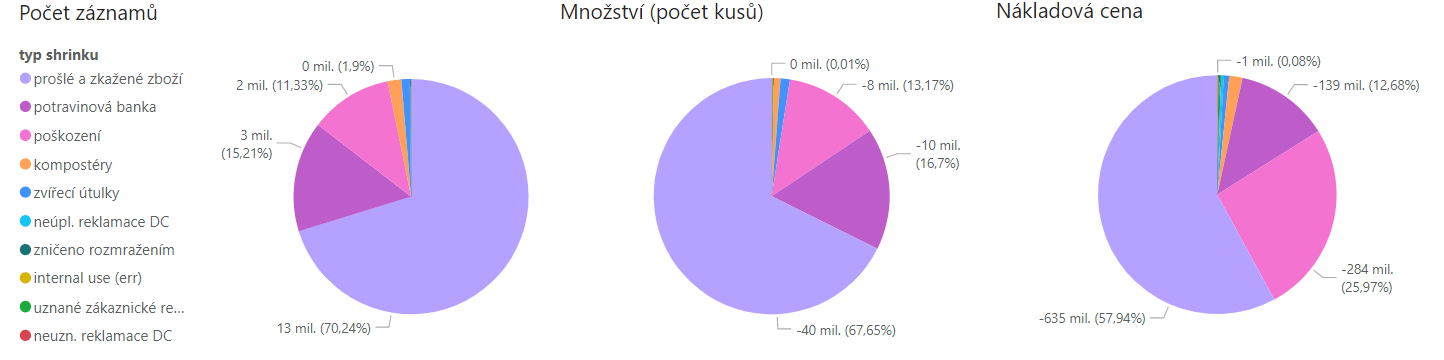
\includegraphics[width=\textwidth]{obrazky/grafy/Graf_celkem-D.png}
    \caption{Znázornění dvou hlavních komponent na dvoudimenzionálních datech.}
    \label{obr:met:PCA1}
\end{figure}


Získání předpisů pro další hlavní komponenty je analogické. Obecně lze zapsat metodu PCA a převod původních proměnných následujícím maticovým zápisem
\begin{equation}
    \mathbf{Y} = \mathbf{XA}, 
\end{equation}
kde $\mathbf{X}$ je matice vstupních dat, $\mathbf{A}$ je matice vlastních vektorů kovarianční matice $\mathbf{C}$. Pro matici $\mathbf{A}$ zároveň platí $\mathbf{C} =  \mathbf{A} \mathbf{\Lambda} \mathbf{A}^\top$, kde $\mathbf{\Lambda}$ je diagonální matice vlastních čísel $\mathbf{C}$.\cite{bib:PCA2}  %wikipedia
